\documentclass{UoYCSproject}
\usepackage{outlines}
\usepackage{tikz}
\usepackage{booktabs}
\usepackage{graphicx}
\usepackage{subcaption}
\usepackage{amsmath}
\addbibresource{bibl.bib}
\author{Angel Simeonov}
\title{Networks and Dragons: A data-driven approach to procedural dungeon generation}
\date{2020-January-27}
\supervisor{Dr. Rob Alexander}
\BEng

\dedication{<insert dedication>}

\acknowledgements{
  <insert acknowledgements>
}

% More definitions & declarations in example.ldf

\begin{document}
\pagenumbering{roman}
\maketitle
\listoffigures
\listoftables
%\renewcommand*{\lstlistlistingname}{List of Listings}
%\lstlistoflistings

\begin{summary}
>At most two (2) pages, aimed a non-specialist, knowledgeable authorial peer.
The summary must:
--state the aim of the reported work,
--motivate the work,
--state methods used,
--state results found, and
--highlight any legal, social, ethical, professional, and commercial issues as appropriate to the topic of study (if none, then this should be explicitly stated).
\end{summary}

\chapter{Introduction}
\label{cha:Introduction}

\section{Role-playing games}
%\begin{outline}
%  \1 Nature and goal  RP is trying to create a compelling narrative in which players can be involved in.
%    \2 Contextualise RPs by comparing different genres. Digital vs Tabletop.
%  \1 Interaction mechanisms. How the game is played and what is the role of the DM
%  \1 Problems: DM has to create the narrative. Can we devise an algorithm that helps DMs create a compelling narrative?
%\end{outline}

\paragraph{}
Role-playing game (RPG) is a broad term encompassing a multitude of different games with often distinct mechanics and platforms of interaction (the media). The common factor between all RPGs is that the player(s) portray a fictional character and is involved in a fictional world (or a subset of one). The interaction of the players with this world is governed by rules, defined by the media. To better understand the structure of RPGs, we can view it in terms of two sets: 
\begin{outline}[enumerate]
  \1 Rules defining how we play the game. Describe the allowed actions for the player at any given moment in the game.
  \1 Narrative elements. Provide the \textit{purpose} of the players to interact with the fictional world. 
\end{outline}
The first set can be viewed as "How I interact with the environment" (functional) and the second as "What is the meaning of the environment" (narrative).

\paragraph{}
Computer RPGs like the Action RPG (ARPG) Legend of Zelda, Diablo, Fallout and many alike have both sets of rules defined by the game designers. A functional rule in an RPG like Skyrim is that you can attack with the left mouse button and a story element is that you are a Dragonborn with a quest. This quest is defined by the writers and designers of the game and as such exploring the narrative in a digital RPG can be comparable to an interactive reading of a fiction book. Good computer RPGs often have the ability to relax the narrative \parencite{TychsenGM}, allowing for the player to have more freedom in the exploration of the world and as such create the sensation that the player has some impact on this pre-programmed fictional environment.

\paragraph{}
The ability for a player to influence the narrative is one of the defining features of tabletop RPGs (TRPG a.k.a pen-and-paper PnP) like Dungeons and Dragons \parencite{DnD}. In them, the functional rules are usually defined by a rulebook (like the Player’s Handbook) and players verbally describe their interactions with the environment. The narrative is an ever evolving amalgam between the input of players and the Dungeon Master (DM). The DM’s task is to create a narrative outline and guide the player interaction. Because of the verbal nature of the game, the narrative does not suffer the limitations of its digital counterparts. But because there are no hard constraints to how the narrative is told, the DM has the non-trivial task of introducing consistency and outlining a structure for the story that would result in a compelling and ideally immersive experience for the players. This is often achieved by focusing the adventure’s act on a particular and detailed location. These locations are often referred to as Dungeons and in practice can be anything from the villain's mansion or a beast’s cave to a city under siege. A good dungeon design is crucial for creating a compelling narrative. The creative task of making the Dungeon is a laborious process. To facilitate that, academics and various gaming communities have been exploring different ways of automating Dungeon creation. We will refer to this process as Procedural Dungeon Generation (PDG). Arguably the greatest problem posed by automating PDG is answering the question of “What is a compelling Dungeon?”. In the next section we will review different generative methods for Dungeons and their associated limitations in an attempt to answer this question.

\section{State of the Art Generative methods}
% \begin{outline}
%   \1 Review various different algorithms for PDG and discuss their take on solving the "is this dungeon interesting?" problem.
%     \2 Non-digital: [[the Advanced DnD DM design kit book 3: Adventure Cookbook]]. Using dice tables to create different elements of the dungeon. Laborious process which requires the DM to remove any inconsistencies. Does not provide an actual Dungeon structure.
%     \2 Cellular automata: donjon \parencite{donjonPDG}. Issues associated with completely random topology and random content generation. Evaluated only on if the level is solvable (no evaluation of semantic content).
%     \2 Constraint Propagators and their related issues when formalising narrative as constraints.
%     \2 BPTs + semantic additions[[citation needed Thrall and Brown]]. Difficulty proving the 'goodness' of the generator. Discuss difficulties with an objective HCI evaluation for PnP (i.e. difficult to get a decent sample size, because playing a game is time consuming).
%     \2 Formal language approach. Grammars \parencite{DormansMS,Deery,Cadogan} as a natural way of describing narrative structures.
%     \2 Data-driven approaches. \parencite{SummervilleLearningOfZelda,SummervillePCGML,SummervilleSamplingHyrule} Relate the notion of learning from human-made dungeons as a way to create good structure + narrative. Note the lack of data. Expand more in the Mission and Space --> Aim sections
% \end{outline}

\subsection{Non-digital Generators}
\paragraph{}
The designers of the classic PnP modules acknowledge the issue of Dungeon creation and often incorporate \textit{Loot} or \textit{Encounter} tables in the rule-books. The tables are a reference over a set of treasures or monsters respectively, which can be chosen by rolling the specified die \textbf{need figure of loot/encounter table}. As noted before, a PnP RPG can evolve rapidly outside the planned narrative structure prepared by the DM and a simple way to quickly define new adaptive story elements via a loot table can be useful. Some early modules even provided a step-by-step guide for creating a full campaign from the plot, villains' obsessions and story setting to the various encounters and and treasures \parencite{ADnD} entirely based on randomised content tables. An issue arises when using loot tables when a randomly selected element from one table is contradicted by an item selected from another. \textbf{show an example from the ADND module}. It is up to the DM to resolve such disparities. As can be seen, this process although providing some degree of creative assistance, it does little to facilitate the laborious nature of creating elements for a compelling narrative. Furthermore, these methods pay no attention to providing guidance of what would mean a good Dungeon as they are occupied with solving global narrative questions. \textbf{Argue that DMs know what they want to do, they just need a facilitator that will create a dungeon based on their requirements ? citation needed for what people use dungeon generators for.}

\subsection{Digital Generators}
\paragraph{}
It is important to note that PnP RPGs and the various genres of computer RPGs although differing in the mechanisms of interaction, they share the same narrative goal \parencite{Tychsen2006}. Therefore we will not limit ourselves to looking only at existing tabletop solutions.
Unlike the original non-digital generators, computerised ones rarely allow for human input in the middle of the process. A generative algorithm would provide a DM with an interface that takes a set of parameters and produce a template of a game. The degree of complexity of this template is naturally dependent on the complexity of the algorithm itself. Because they aim to exclude the human designer from the process, the digital generators tend to focus on creating elaborate Dungeon spaces and struggle providing coherent semantic content \parencite{Thrall,Brown}.

\subsubsection{Cellular Automata}
Cellular automata (CA) utilises a procedural generation mechanism in which a $N \times M$ grid space is mutated incrementally by a set of agents\textbf{[citation needed for CA and fig. showing agents in action?]]}. The implementation of these mutation operators define if the CA will simulate erosion \parencite{donjonCA} or man-made structures such as rooms and corridors. The latter is the case of the donjon dungeon generator \parencite{donjonPDG}. Its simplicity and degrees of customisations of both layout and style has made donjon a popular generator choice with more than 2500 generated dungeons in the last 12 hours and 100 donations in the last 3 months \textbf{[[citation needed?]]}. Despite its popularity, donjon (as well as other CA) implores purely random generation techniques which are only evaluated based on a notion of the solvability of the level. The criteria for donjon's level is only if each room is reachable (i.e. there is a path to each room). As it can be observed, although we have control over the input parameters for the topological randomness, the semantic elements (the contents, rather than the structure) of the dungeon are entirely arbitrary and often contradictory \textbf{[[citation of brown and thrall or elaboration?]]}. In terms of the aforementioned solvability, when accounting for reachability donjon does not take in account the randomly allocated locked doors as the key allocation is left at the DM's discretion. That ultimately limits the usefulness of the tool and only provides a skeleton for the dungeon. All information generated about the monsters, treasures and other quest elements are discarded by the DM \textbf{[[citation needed on how people use dungeon generators]]}

\subsubsection{Constraint Propagators}
Constraint Satisfaction Problems (CSPs) define a discrete set of variables with corresponding constraints that restrict the possible variable instantiations \textbf{[[cn  of CSPs]]}. Dungeon generation has been described as a CSP on occasions where the variables and constraints define the layout \textbf{[[cn]]}, contents \textbf{[[cn]]} or both layout and content\textbf{[[cn]]} of a dungeon. Constraint Propagation (CP) is a particular method proven useful for solving CSP in the context of dungeon level generation. The algorithm selects a set of possible values for a particular variable and \textit{propagates} the result to the rest of the variables, adjusting their possible values accordingly. If the selected value narrows another variable's possible values to the empty set, we infer that this instantiation is suboptimal and we backpropagate to the last viable solution and retry. Furthermore it can be generalised that if an instantiation for all variables that does not narrow any variable to the empty set exists, the level is solvable. Utilising this formalisation of the \textit{solvability} of a level we can populate a level with varying degrees of complexity from ensuring that keys are always spawned before the door that they must unlock to adjusting difficulty by measuring survivability metrics between rooms \textbf{[[cn]]}. Even thought CPs have solved some problems of the completely random generators, formulating a numerical constraint for a narrative element can be difficult. The complication is both in the translation of a story element to a numerical representation and in the computational expense that comes with computing large amounts of permutations.

\subsubsection{Binary Partitioning}

\subsubsection{Formal Languages}

\subsubsection{Data-driven approaches}

\section{Mission and Space}
% \begin{outline}
%   \1 Introduce the notion of Mission and Space
%   \1 The reason for separating Mission and Space. We can model player experience better \parencite{DormansMS,SummervilleLearningOfZelda}.
% \end{outline}

\paragraph{} %ToDo: Finish Mission & Space Argument. Why do we have this section? insert a fig of Dormans Mission to Space mapping ??
An attentive reader would have noted that distinguishing between the level layout and contents is a common occurrence in popular PDG algorithms. This discrimination was formalised by Dormans\parencite{DormansMS} in his definitions of \textit{Mission} and \textit{Space} in relation to the ARPG Legend of Zelda game series.
The \textit{Space} of a dungeon embodies it's topological structure and can be encoded as an undirected cyclic graph where each vertex is a room and each edge is a door or corridor. The \textit{Mission} is the set of narrative tasks the player must accomplish in order for him to complete the dungeon. It can be encoded as a directed graph where each vertex is the objective and the edge directions show the required sequence of completion. It is clear to see that the gameplay experience is defined in the interaction of the two graphs. As noted by Dormans, a \textit{Mission} mapped on different layouts will result in drastically different exploration patterns and it is by understanding the necessities of the two separate entities that we can model player experience better. Due to this separation we have seen advancements in generating adaptable to the player game environments \parencite{DormansAE} and even reverse engineering the creation of \textit{Missions} and \textit{Spaces} by learning structure from data \parencite{SummervilleLearningOfZelda}.

\section{Aim}
%\begin{outline}
%  \1 The only \textit{"dungeon generator"} that has been empirically proven to have the ability of creating a truly compelling narrative is the human designer
%  \1 Discuss attempts at the data-driven approaches from \textbf{Generation Methods} in detail
%    \2 Deery's data inspired approach, but not data-driven
%    \2 Summerville's Learning of Zelda
%\end{outline}

\paragraph{}
The dungeon’s topology (Space) and contents (Mission) are correlated and embody the narrative of the game. As we have seen, dungeon generators usually implore bottom up approaches in which they apply rules for topology and then introduce dungeon content in an attempt to provide the structure for a captivating narrative. The various algorithmic methods have clear strengths and shortcomings in achieving the complex goal of creating an interesting story. I want to argue that from these observations we can affirm that the ultimate \textit{dungeon generator} is the human designer. Dungeons and therefore narratives produced by humans are the most compelling out of all created dungeons. As noted by others \textbf{[[cn]]}, if we implore a top-down approach of analysing what makes a good man-made dungeon, we could potentially achieve higher levels of narrative automation.
\paragraph{}
Deery made the first steps by manually analysing submissions to the One Page Dungeon Contest \textit{OPDC} \parencite{OPDC} to extract a graph grammar for Mission generation \parencite{Deery}. The Mission graph was then mapped to a physical Space in a 1:1 ratio. The result was that each room was limited to a single Mission element. It is trivial to see that the originals in OPDC do not impose such a restriction. One room can have multiple Mission elements (e.g. the key to unlocking the door is on the bandit’s waist, Key + Encounter). Furthermore, Deery’s approach was to manually look at 10 competition winners and heuristically extract the grammar rules, which he highlights that they do not capture all the possible patterns. An automated approach to learning would potentially solve that issue. Programmatically learning a level from data has been an object of interest for computer based RPGs \parencite{SummervilleLearningOfZelda}, but has not been applied to PnP RPGs, presumably because of the lack of a consistent dataset.

\paragraph{} % TODO: make this more succinct and make the goal clear: this model has successfully mimicked a human authored dungeon. We establish this 
In this paper we will investigate if applying a data-driven approach to learning the Space of the dungeon can produce a map that is undistinguishable from human-made dungeon topologies. We will define a meaningful set of features to be extracted from the OPDC dataset and use those features as random variables defining an Inference (Bayesian) Network. Subsequently we compare different network structures and learning algorithms and internally assess which model has the greatest statistical predictive capabilities using various scoring rules. We will use the best model to generate a dungeon and conclude with a user study to externally validate how well the generator has approximated human-made dungeon topologies. %We will discuss how we convert from sample to dungeon, concluding by using a Mondrian study to externally validate if our model is able to generate topologies that are indistinguishable from human-made  

% In this paper we will investigate if we can use the OPDC dataset and apply a data-driven approach of sampling an Inference (Bayesian) Network to create the layout of a small (one session long) dungeon. We will first explore the availability of data and the selections of parameters we want to learn. We will discuss the choice of using inference networks for our generator. Then we will do a comparative analysis of different graph structures and algorithms for fitting our parameters. The comparison will be based on our internal validation Scoring Rules \parencite{PearlScoringRules} assessing which model has the greatest statistical predictive capabilities. We will conclude by externally validating our best model’s capability to create human-like topologies with a user study.

\chapter{Bayesian Inference Networks}
\paragraph{What are Bayesian networks?}
Bayesian Networks \textit{BNs} \parencite{pearl1985bayesian} (also referred to as Inference Networks, Belief Networks or Directed Acyclic Graph \textit{DAG} Models) are a graphical probabilistic model in which vertices are random variables \textit{RVs} whose edges indicate causal beliefs. BNs assert that our domain is defined in terms of a joint probability distribution \textit{PD} \(P(X_1, \ldots , X_n)\) over a finite set of RVs \(X\), each of which has a set of potential values it can take \(X_i(\Omega) = \{x_1, \ldots, x_j\}\) with an associated PD. The network structure shows how the full join distribution factorises given the causal dependencies. This property gives us a way to encode our prior domain knowledge about the relationships between our RVs.
Once we have encoded the RV interaction, using a BN as an inference tool is a matter of querying with a conditional set of RVs and noting how the conditional probability tables \textit{CPTs} change given our new knowledge. In practice, conditioning is done by \textit{observing} (i.e. instantiating) an RV to be a particular value. Extracting information from our newly formed conditional distributions is done by sampling. Sampling involves simulating our network with respect to the observations in order to obtain point estimates. A detailed discussion of the sampling methodology will be provided in section \ref{sec:implementation}.

To contextualise the inference process, we can look into Summerville's work on the Legend of Zelda dungeons \parencite{SummervilleLearningOfZelda}. After annotating the dungeon maps with elements of both Mission and Space (total number of rooms, treasures, monsters, critical path CP, etc.), he extracts features for the BN by parsing them as RVs. If we condition on total number of rooms (i.e. observe \(P(NumRooms = n) = 1\)), the PD for the possible CP would reflect our new knowledge. Most likely the CPs that are greater than the total number of rooms would be impossible \(P(CriticalPathLength > n \mid NumRooms = n) \rightarrow 0 \), which is logical. Then by sampling the network we can get a point estimate for critical path length given that number of rooms in the dungeon. This \textit{observe-then-infer} process can be done with any permutation of our RVs.

\paragraph{Why use Bayesian networks?}
% causal structures gives us a natural interpretation of complex non-linear problems, compared to other methods (think NNs and their inability to be interpreted)
% they are fast once trained. Updating belief is a simple arithmetic operation on the different CPT
% gives us precise control over the parameters. Deery had an approximation of how big a dungeon should be because he would just repeat the rules X number of times. We can precisely fix every parameter that we have and even do permutations. This gives new degrees of freedom for the user to select the desired properties of his dungeon without compromising on automation.
The reasoning behind choosing BNs is that the probabilistic causal structures have been shown to perform well in capturing properties from data for PDG tasks in ARPGs \parencite{SummervilleLearningOfZelda,SummervilleSamplingHyrule}. Furthermore they give us a natural description about the dependencies in our model, which can be used as a supplemental analysis tool for investigating human-made dungeons. As a PDG tool itself, the \textit{observe-then-infer} pattern gives the user precise control over the desired properties of his dungeon without loss of automation. If a user observes a dungeon with 5 rooms and critical path of length of 3, they will be guaranteed in the final product. This solves the problem previous graph grammar data-driven approaches encountered, whereby the dungeon size input was used as an approximation for the actual number of rooms in the dungeon \parencite{Deery}.

The downside of BNs is that their generalisation capabilities are highly dependent on the availability of data. If conditioning on an undefined set (e.g. there was never a data entry that showed a 5 room dungeon with CP of 3), the inference will fail. A proposed way to solve this issue is by creating artificial data entries for the undefined cases. We will use linear interpolation due to its simplicity and the fact it has been shown to produce good results in general \parencite{Ibargengoytia2013OnTE} and exceptional results on small datasets \parencite{yu2004advances}. This can potentially solve the problems of undefined dungeons within the range of sizes of our dataset, but it cannot extrapolate to infer arbitrarily large dungeons. We would argue that that generalisation is not necessary as we are trying to capture properties of One-Page dungeons which are designed to be small enough to be fit in a single gameplay session. 

% \paragraph{What we need to do to use Bayesian Networks?}
% We need to define two key attributes of the BN:
% \begin{outline}[enumerate]
%   \1 The causal structure
%   \1 Conditional probability tables \textit{CPTs} for each RV
% \end{outline}
% In this paper we will apply an empirical approach and evaluate different models in search of the model with highest statistical predictive capabilities. In section \ref{sec:model_selection} we will compare in detail two structures with three CPT learning algorithms for a total of six models. The structures are the previously proposed Extreme Sparse model \parencite{SummervilleSamplingHyrule} (modified for Space only) and an automatically learned structure using the Tree Augmented Na\"{i}ve Bayes. The CPT learning algorithms will be a simple joint occurrence count, Expectation Maximisation \textit{EM} and Gradient Descent \textit{GD}.

\chapter{Methods and Implementation}
\section{Data acquisition}
\subsection{Data selection} % what dataset should we choose:: OPDC winners for the last five years
% What problems can we encounter? Sparsity of data. Very different dungeons, some are unusable (say unusable criteria)
\paragraph{}
Unsurprisingly the first priority of a data-driven method is the acquisition of a suitable dataset. The criteria we have chosen for our data is the following:
\begin{outline}[enumerate]
  \1 Data must be consistent. Dungeons have to be representatives of a similar and comparable category.
  \1 Data must be available under a research or similar open-source license.
\end{outline}
The \textit{OPDC} supplies a dataset that satisfies our requirements. All dungeons are in the same category of a one-session long dungeon and each dungeon is issued under the Creative Commons CC license. Furthermore due to the fact that it is a competition, we have an exemplar answer of our main question "What makes compelling dungeon?" in the form of the competition winners. We apply the first filter and review only entries by competition winners. Due to the creative freedom the human designers have, it is na\"{i}ve to assume that the dungeon Space is necessarily a dominant factor in all dungeons. In order to narrow down to dungeons that do have a consistent representation of Space as an important asset, we apply a second filter by omitting dungeons that have:
\begin{outline}[enumerate]
  \1 exclusively linear topologies
  \1 no map (no Space)
  \1 non-standard Space traversal (the map topology is ignored due to a functional mechanism e.g. time-travel, game of political control, king of the hill, etc.)
  \1 inconsistent map (our Space parameters are allowed to change e.g. intrigue campaigns where the objective constantly changes locations)
  \1 no goal defined by the designer (introduces the same problem as 4.)
\end{outline}

\subsection{Extracting Features}
\paragraph{}
We will base our feature selection on the work done by Summerville \parencite{SummervilleSamplingHyrule} by selecting Space related parameters from his Extreme Sparse model due to its simplicity and effectiveness. We extract five parameters in two categories: 
\begin{outline}[enumerate]
  \1 Dungeon (Global): total number of rooms \(R\) and how many rooms are on the critical path \(C_{length}\)
  \1 Room (Local): depth (how far away the room is from the entrance) \(D\), critical path distance (how far away is the room from a critical path room, 0 indicates it is on the CP) \(C_{dist}\), total number of neighbours \(N\)
\end{outline}
Each global and local set of parameters is defined by the joint PDs respectively \(P(R, C_{length})\) and \(P(C_{dist}, D, N)\). A full dungeon is therefore characterised by \[P(R, C_{length}) \prod_{i=1}^{\mid R \mid} P(C_{dist_i}, D_i, N_i)\] where \(|R|\) is the total number of rooms defined by the instantiation of \(R\). To extract the five parameters, we need to transform the artistic and graphically rich textual representations of dungeons in our dataset. Unfortunately automating feature extraction is very difficult due to the variant stylistic formatting and the prose like description of the tasks. Because of this, we establish a systematic way of manually annotating the Space of the dungeon as an abstract undirected graph from which we can calculate all the different parameters as shown in \textbf{[[insert figure of 2015 Sepulchre of the Abyss transcriptions]]}.

\paragraph{}
\textbf{TODO: Filling in the data gaps. Linear interpolation and artificial datapoints}

\paragraph{}
The final dataset is saved in a CSV format and consists of \textbf{[[size]]} organic entries and \textbf{[[synthetic]]} linearly interpolated entries for a total of \textbf{[[dungeon params]]} and \textbf{[[room params]]} with dungeon sizes ranging from [\textbf{[[min]]-[[max]]}] rooms. %ToDo: insert statistical figures about the dataset. Histograms of the different features, mean, variance and lower/upper bounds.

\section{Model selection} % we have to choose a model structure denoting assumptions about dependencies then compute the CPTs
\label{sec:model_selection}

\paragraph{What we need to do to use Bayesian Networks?}
We need to define two key attributes of the BN:
\begin{outline}[enumerate]
  \1 The causal network's topology
  \1 Conditional probability tables \textit{CPTs} for each RV
\end{outline}
In this paper we will apply an empirical approach and evaluate different models in search of the one with highest statistical predictive capabilities. We will compare two structures with three CPT learning algorithms for a total of six models. The structures are the previously proposed Extreme Sparse model \parencite{SummervilleSamplingHyrule} (modified for Space only) and an automatically learned structure using the Tree Augmented Na\"{i}ve Bayes. The CPT learning algorithms will be a simple joint occurrence count, Expectation Maximisation \textit{EM} and Gradient Descent \textit{GD}. Implementation of all BN related algorithms is done in the Netica Bayesian Network development software \parencite{netica}.

\subsection{Bayesian Network topology}
\subsubsection{Summerville's Extreme Sparse Model \textit{SESM}}
In exploring data-driven PDG for the Legend of Zelda franchise, Summerville found out that when dealing with a small dataset (38 dungeons with 1031 rooms), the SESM is able to capture high level properties of both Mission and Space with the highest accuracy in respect to the learning criteria and the lowest complexity. Following our assertion that digital RPGs differ from PnP RPGs only in mechanisms of interaction, we will base one of our BN topologies on Summerville's work. In order to do so, we flatten down the graph to use only the Space parameters we have extracted from the OPDC data. The flattening is done by reconstructing the SESM in Netica and applying the \texttt{AbsorbNodes\_bn} \parencite[62-63]{neticaCman}. The function removes the unused Mission RVs by effectively treating them as constants and propagating any implied dependencies from the other nodes. In this way we remove the unused RVs and maintain the joint distribution dependencies between our Space parameters. The transformation can be seen in figure \ref{fig:SESM}. The resulting model describes the following factorisation over our RVs

\[P(R,CP_{length},CP_{dist},D,N) = P(R)P(CP_{dist})P(CP_{length} \mid R)P(D \mid R, CP_{length})P(N \mid D, CP_{dist})\]

Ignoring Mission parameters does reduce the dimensions of the model and can potentially reduce predictive capabilities.
% Summerville applied a BNet approach to learning levels of the ARPG game Legend of Zelda. As noted before, digital RPGs differ from PnP RPGs only in mechanics of interaction and therefore we can cautiously analyse his findings. He found out that for limited amounts of data (\textbf{[[insert his dataset size]]}) a sparse model is able to produce the highest factor of learning against a Bayesian Informational Criterion (BIC). His network structure includes both Space and Mission parameters \textbf{[[fig of sparse model]]}. We don't need that because X. We apply vertex absorption, which removes the unnecessary nodes whilst preserving global conditional dependencies. We can do this because in our case we can treat the unused Mission nodes as constantly observed and not giving us any new dimensions to explore. The adapted sparse DAG from Summerville can be seen in \textbf{[[fig of PnP Inference DAG]]}

\begin{figure}[htb]
  \centering
  \begin{subfigure}[b]{0.55\textwidth}
    \centering
    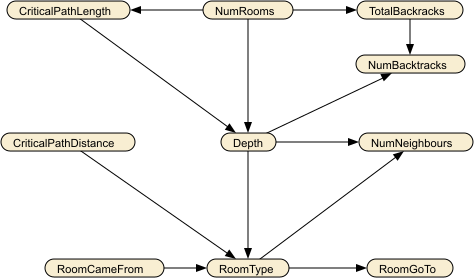
\includegraphics[width=\textwidth]{SESM_full.png}
    \caption{Sumerville's Extreme Sparse Model}
  \end{subfigure}
  \hfill
  \begin{subfigure}[b]{0.35\textwidth}
    \centering
    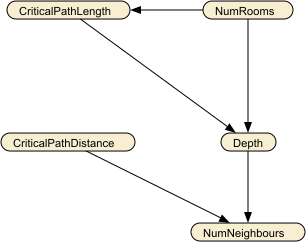
\includegraphics[width=\textwidth]{SESM_space.png}
    \caption{Space only Model}
  \end{subfigure}
  \caption{Bayesian Network topologies in Netica}
  \label{fig:SESM}
\end{figure}

\subsubsection{Tree Augmented Na\"{i}ve Bayes}
% In the above approach we used specialist knowledge (Sumerville's experiments) to create the BN structure
% We made two crucial assumptions in that PnP == ARPG && flattening Mission to Space only will still retain the same operational meaning of the dungeon due to it retaining the same conditional dependency assumptions through the BN properties
% But we want to put those assumptions to the test by also learning the graph structure from the data we have.
\paragraph{}
In the above approach we applied specialist knowledge from Sumerville's experiments to create the BN structure. For that network to be valid, we asserted two assumptions about equivalence between PnP and ARPG dungeons and that flattening Mission to Space retains the same operational meaning due to the BN retaining the same conditional dependencies. To contest these somewhat ambitious assumptions, we will also create a BN by ignoring any domain knowledge we have and infer the structure purely based on the data using Netica's Tree Augmented Na\"{i}ve Bayes \textit{TAN} \parencite{FriedmanTAN}.  
\paragraph{}
Informally the learning procedure can be defined as finding the most likely BN structure that agrees with our data. The TAN algorithm starts with the usual na\"{i}ve Bayes model structure which states that all RVs are conditionally independent given one specific RV (the class RV). We will choose the class to be \(R\) \textbf{[[Elaborate why. Correlation with the restriction on the conditioning set]]}. The na\"{i}ve assumption implies that \[P(R,\boldsymbol X) = P(R)\prod_{x}^{\boldsymbol X} P(x \mid R)\] where \(\boldsymbol X = \{C_{length}, C_{dist}, D, N\}\). With this very restrictive assertion we, in practice, have a BN structure that we can use. But although the induced bias towards the class is often shown to be practically useful, in our case assuming that the room parameters are independent from each other does not make much sense. For precisely this reason, the TAN algorithm analyses our data and creates \textit{augmenting edges}. They are causal links connecting RVs that are found to have correlations. The final structure which can be seen in \ref{fig:TAN} is the original na\"{i}ve Bayes with the extra added augmenting edges, resulting in a model that has a moderated bias factor for the class and an informed causal structure. It should be noted that the we did not discuss the \textit{tree} nature of TAN, because it is related to practical optimisations for learning large graphs. We are not concerned with this as our model contains only five RVs.

%The convenient restriction we imposed early in the paper of only conditioning on \(NumRooms\) was so that we have a clear candidate for this class variable. 
%TODO: GET ALL THE DATA AND PUT IT HERE
\begin{figure}[htb]
  \centering
  \begin{subfigure}[b]{0.55\textwidth}
    \centering
    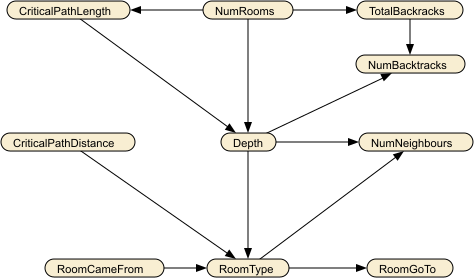
\includegraphics[width=\textwidth]{SESM_full.png}
    \caption{Na\"{i}ve Bayes}
  \end{subfigure}
  \hfill
  \begin{subfigure}[b]{0.35\textwidth}
    \centering
    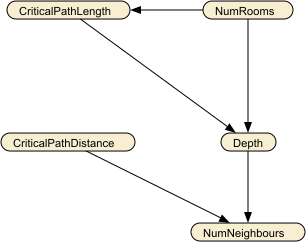
\includegraphics[width=\textwidth]{SESM_space.png}
    \caption{TAN}
  \end{subfigure}
  \caption{Bayesian Network topologies in Netica}
  \label{fig:TAN}
\end{figure}


\subsection{Parameter Learning}
\subsubsection{Count}
\subsubsection{Expectation Maximisation EM} %both EM and GD can get stuck on local minima
\subsubsection{Gradient Descent GD}

\section{Implementation}
\paragraph{}
The platform of choice for this project is .NET with the language of implementation being C\#. We chose this as Netica has native support for C\# via its COM API and because of the availability of useful third-party utilities. Namely we will be using Nepo\v{z}itek's PDG tool \parencite{levelGenerator} which allows us to input an abstract graph for the desired topology and produces a rendered image that is ready for player usage. The reason behind using a third-party solution for the dungeon rendering is due to time constraints and the fact that the visualiser is not a centre piece of this experiment. Our sole requirements are that the rendering is consistent and robust enough to handle our produced topologies. Nepo\v{z}itek's PDG satisfies these requirements \parencite{Nepozitek2018FASTCT}.
\label{sec:implementation} %from chosen model --> dungeon graph, assumptions about constraints specifics etc
\paragraph{Dungeon Sampling} %What 
We can define characteristics of the desired dungeon by leveraging the inference nature of BNs. Generating a dungeon with five rooms is a matter of fixing (\textit{observing}) the \texttt{NumRooms} parameter. The user can choose virtually any permutation of parameters to be fixed or inferred. For consistency of this experiment, we are observing only the size of the dungeon via \texttt{NumRooms}.

\paragraph{Room Sampling}
% fix dungeon, sample the rest
% Netica applies the Naive Bayes assumption that given the class variable NumRooms, all rooms are independent. The reason for this assumption is that we avoid the computational complexity of maintaining series of CPTs for each room instantiation. Why is this assumption not bad for us? Potentially because it's empirically shown to not decrease accuracy? https://www.norsys.com/WebHelp/NETICA/X_Bayesian_Learning.htm "Assuming the conditional probabilities to be independent generally results in poor performance when the number of usable cases isn’t large compared to the number of parent configurations of each node to be learned." We're safe because the ratio from parent (dungeon params) to children (room params) is count(dungeon.csv)/count(room.csv)

\paragraph{Converting from samples to Space}
%considerations.
%Propositions:
%1. Ad-hoc implementation : not pretty, cannot guarantee its valid without assuming soft constraints
%2. Heuristic search ==> I could not conceptualise an intuitive way to use search. Search over the space of potential room connections. The heuristic is going to be a production of the sampled parameters (sounds like CSP with an extra step?)
%3. Graph grammars  
% + intuitive, just apply graph production rules until we satisfy the sampled params.
% - Not extensible, if we create a representation now for Space, if we want to extend it to include Mission parameters we have to make the graph typed, which is not a trivial thing to do.
% - Our production rules (grammar) will be heuristically created.
%4. Constraint solvers
% + intuitive, the sampled params are our constraints.
% + Extensible: if expanding to Mission, we just add new constraints to be satisfied.
% + gives us an intuition about solvability, which is a bonus internal metric for our BNet. I.e. did we sample something that makes sense? 
% + can be generalised and optimised :: potentially translate it for general linear solvers

\chapter{Results}
\label{cha:results}
\section{Internal Validation}
\begin{table}[htb]
  \centering
  \resizebox{\textwidth}{!}{%
  \begin{tabular}{@{}llllllllll@{}}
  \toprule
                        & \multicolumn{3}{c}{Count}                                                        & \multicolumn{3}{c}{EM}                                                           & \multicolumn{3}{c}{GD}                                                           \\ \midrule
  \multicolumn{1}{l|}{} & \multicolumn{1}{c}{log} & \multicolumn{1}{c}{quad} & \multicolumn{1}{c|}{sphere} & \multicolumn{1}{c}{log} & \multicolumn{1}{c}{quad} & \multicolumn{1}{c|}{sphere} & \multicolumn{1}{c}{log} & \multicolumn{1}{c}{quad} & \multicolumn{1}{c|}{sphere} \\ \midrule
  Extreme Sparse        &                         &                          &                             &                         &                          &                             &                         &                          &                             \\
  TAN                   &                         &                          &                             &                         &                          &                             &                         &                          &                             \\ \bottomrule
  \end{tabular}%
  }
  \caption{Structure and parameter learning comparison.}
  \label{table:BNetCompare}
  \end{table}

\section{External Validation} %user study

\chapter{Discussion}

\section{Critique}
\begin{outline}[enumerate]
  \1 Data
    \2 availability and extraction. 
      \3 Could extend to include even non-winning entries for the sake of having a greater sample size. More datasets can be considered. We've use OPDC due to its CC license, but paid modules exist.
      \3 Data extraction has been a manual process. Although due diligence is paid, noise introduced from human error is inevitable. 
  \1 Method
    \2 Cannot generalise to unseen cases. We can interpolate for missing data, but we cannot extrapolate. Argue that this is an issue of all ML approaches, not just BNets, because we're trying to capture properties of One-Page dungeon.
    \2 This paper is considering only Space gen. A more robust approach would be needed to extract consistent and meaningful parameters for Mission. For Legend of Zelda there is a discrete subset of things you can do so that is why Mission extraction is possible. Deery has shown that formalising Mission in PnP RPG's is difficult due to the variant and creative nature of the human-made dungeons.
  \1 Validation
    \2 We have decided to approach the external evaluation in a quantitative, rather qualitative measuring. That is due to the fact that conducting a study with a high environmental index is difficult due to multiple confound factors that are due to the nature of a tabletop RPG session. Not only does a one-session adventure usually take around 3 hours \textbf{[[cn]]}, but they are extremely variant between groups of players and DMs. An experiment that analyses how players use the generated dungeon rather than just discriminating between different dungeons topologies would give us more insight in the success of the recreation of a human-made dungeon.
  
\end{outline}

% \begin{figure}[htb]
% \begin{center}
% 
\includegraphics[height=3cm]{"./UOY-Logo-Stacked-shield-Black.png"}
% \end{center}
% \caption{A figure containing UoY logo and its caption.}
% \end{figure}


\chapter{Conclusion}
\label{cha:conclusion}

\subsection{Future Work}
\begin{outline}[enumerate]
  \1 Rerun with more data (OPDC is conducted every year)
  \1 Automate the Feature Extraction process (OCR + NLP)
  \1 Incorporate Mission parameters as well
  \1 Analyse PnP specific dungeons and find more parameters that might be useful. E.g. size of rooms, multiple CPs, 
  \1 Conduct a study with greater environmental impact (e.g. actually get people to play instead of using an aesthetics study)
\end{outline}


\appendix
\chapter{Some appendix}
\textit{Use this section for graphical showing of the models. Nets, result tables (or tables should be inline?)}

\chapter{Another appendix}
\textit{Use this section for questionnaires and external validation support}

\printbibliography

\end{document}